

\documentclass{beamer}
 
\usepackage[utf8]{inputenc}
 
 
%Information to be included in the title page:
\title{Multi-Agent Ethical Planning}
\author{Axel Ind}
\institute{Uni-Freiburg}
\date{\today}
 
 
 
\begin{document}
 
\frame{\titlepage}
%----------------------INTRODUCTION------------------------------------------------
%----------------------------------------------------------------------------------

%----------------------EXAMPLE-----------------------------------------------------
\begin{frame}
\frametitle{Example}
\begin{itemize}
\item Two students (A and B) have a test to study for.
\item They each need a certain textbook from the library. 
\item The library has 2 copies of the textbook, one in English and one in German.
\item Student A speaks both English and German, Student B speaks only English.
\item A arrives at the library early and gets to choose which book he wants first.
\end{itemize}

\end{frame}

 
\begin{frame}
\frametitle{Example: Agent A}
Agent A:
\[
\Pi_A = (V_A, O_A, I_A, \gamma_A, u_A)
\]
\[
O_A = \{ O_{A_{takeEnglish}}, O_{A_{takeGerman}}, O_{A_{doNothing}}\}
\]
\[
O_{A_{takeEnglish}}=(libraryHasEnglish, \lnot libraryHasEnglish \land AhasEnglish)
\]
\[
O_{A_{takeGerman}}=(libraryHasGerman, \lnot libraryHasGerman \land AhasGerman)
\]
\[
O_{A_{doNothing}}=(\top, \top)
\]
\[
I_A = (libraryHasEnglish, libraryHasGerman)
\]
\[
\gamma = (AhasEnglish \lor AhasGerman)
\]

$u_A$: considers ethical evaluation of B's actions.

\end{frame}

\begin{frame}
\frametitle{Example: Agent B}
Agent B:
\[
\Pi_B = (V_B, O_B, I_B, \gamma_B, u_B)
\]
\[
O_B = \{ O_{B_{takeEnglish}}, O_{B_{takeGerman}}, O_{B_{doNothing}}\}
\]
\[
O_{B_{takeEnglish}}=(libraryHasEnglish, \lnot libraryHasEnglish \land BhasEnglish)
\]
\[
O_{B_{takeGerman}}=(libraryHasGerman, \lnot libraryHasGerman \land BhasGerman)
\]
\[
O_{B_{doNothing}}=(\top, \top)
\]
\[
I_B = (libraryHasEnglish, libraryHasGerman)
\]
\[
\gamma = (BhasEnglish)
\]

$u_A$: \textit{does not} consider ethical evaluation of A's actions.
\end{frame}

\begin{frame}
\frametitle{Example: Combined Task}
Combined Task:
\[
\Pi = (V, O, I, \gamma, u, T)
\]
\[
O = (O_A, O_B)
\]
\[
V = V_A \oplus V_B
\]
\[
I = I_A \oplus I_B
\]
\[
\gamma = (\gamma_A, \gamma_B)
\]
\[
u=(u_A, u_B)
\]
$T$: an ordering function to linearise agent actions consistently  (turn taking in this case).
 \end{frame}
 
 
 
\begin{frame}
\frametitle{Flowchart}
\centering 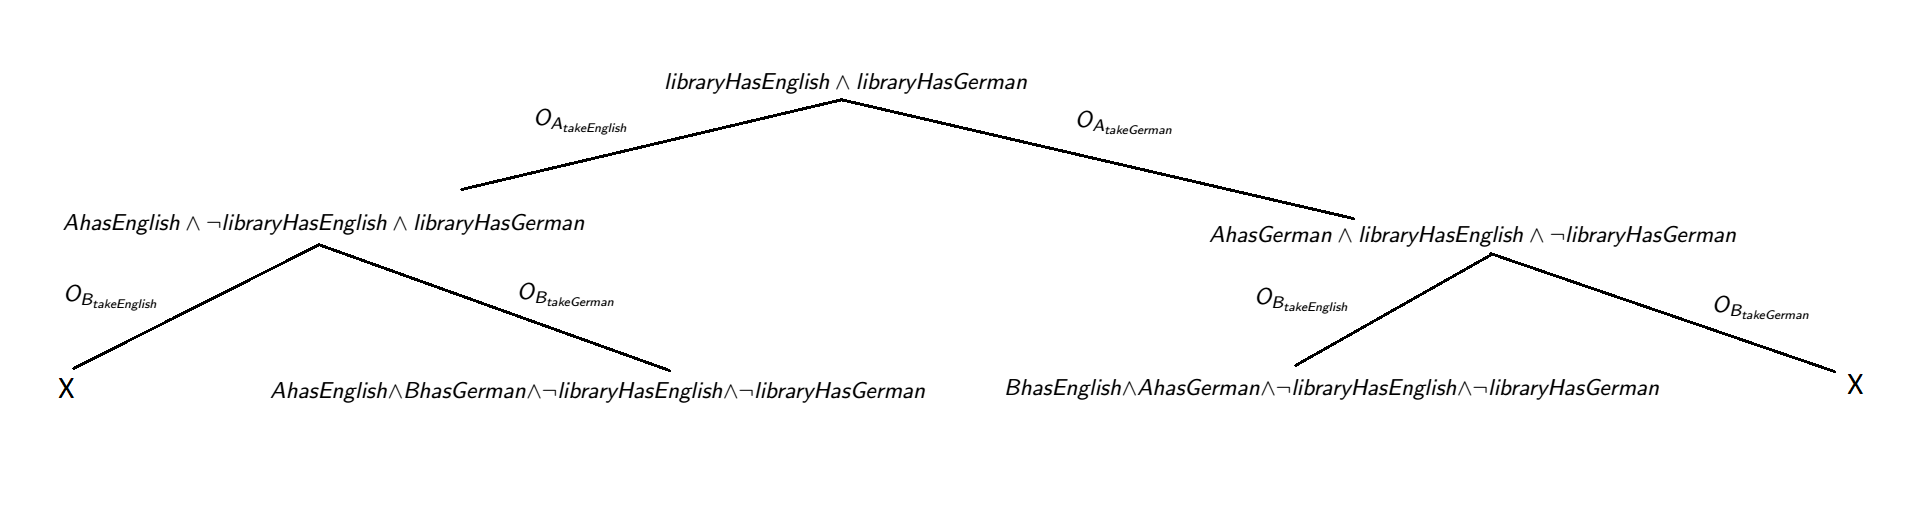
\includegraphics[scale=0.23]{exampleFlowchart}
 \end{frame} 

\begin{frame}
\frametitle{Flowchart}
\centering 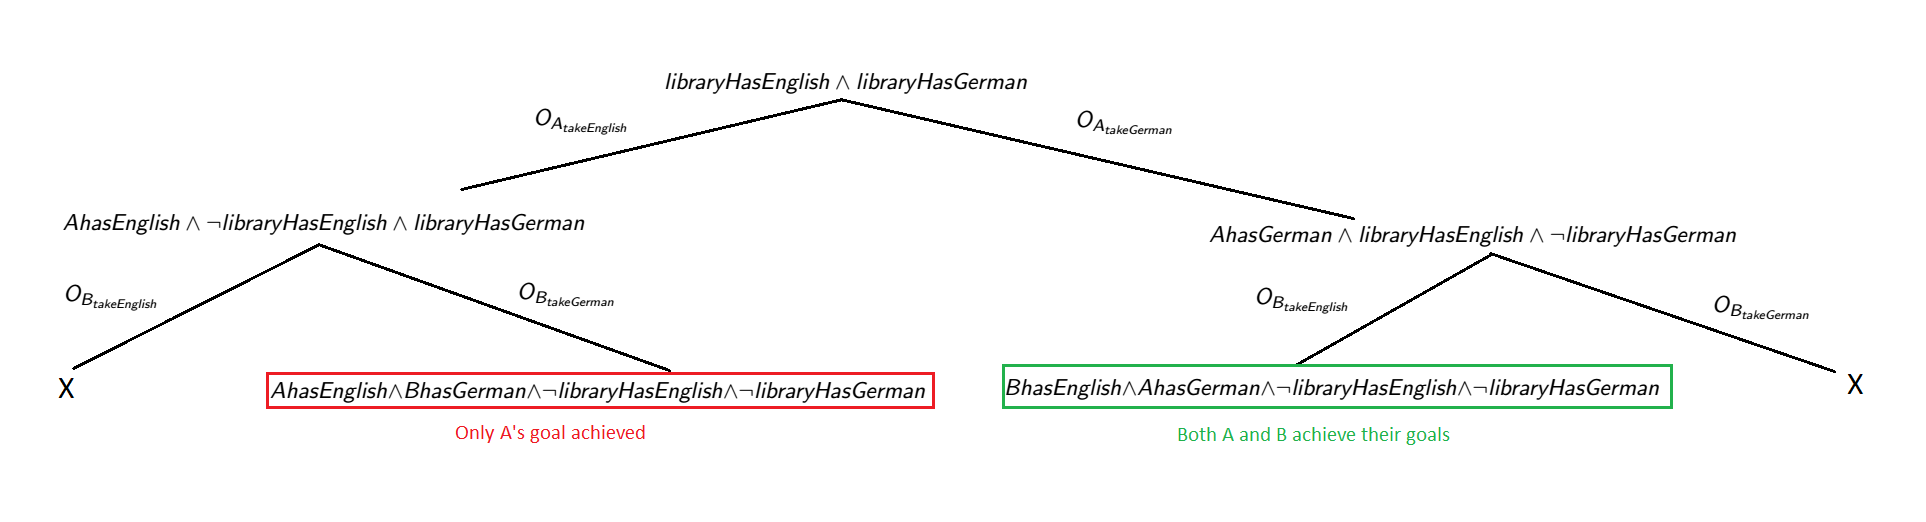
\includegraphics[scale=0.23]{exampleFlowchartAnnotated}

\begin{itemize}
\item Without ethical restrictions of permissable actions, agent A can reach its goal but render agent B's goal unreachable.
\item This is not necessarily bad (e.g. in competitive games), but there are cases where it harms the system as a whole.
\end{itemize}
 \end{frame} 
 
 
\begin{frame}
\frametitle{Deontological Approach}
\begin{itemize}
\item \textit{Actions} labelled \textit{a priori}.
\item Only allow good or morally neutral actions.
\item Morally permissible if: $u(s,a) \geq 0$.
\item For single agent sufficient to simply check if a candidate action has non-negative.
\item For multi-agent case, two possibilities:
\begin{enumerate}
\item Single-agent ethical utility: Consider only the ethical utility of the state-action pair for the acting agent.
\item Agent set ethical utility: Consider ethical utility of the state-action pair of the current agent and \textit{all agents that act after it} until the current agent is able to act again.
\end{enumerate}
\end{itemize}
 \end{frame} 
 
 
 \begin{frame}
\frametitle{Agent Set Ethical Utility}
\begin{itemize}
\item Requires ethical utility labels for other agent actions.
\item If the other agents are random or have unknown $u$, consider worst-case or average-case of their applicable actions.
\item If the other agents $u$ function is known, more complex:
\begin{itemize}
\item If all subsequent agent actions for this turn are morally good or neutral, then the original action is applicable. If all are morally bad or neutral, the action is morally inapplicable. 
\item If both agents follow deontological ethics, and have the same (agent-independent) utility function: it is sufficient to consider the best-case scenario of other agent action selection.
\item In other cases the other agent's actions must be evaluated using their own ethical function to determine what action they will take. Potentially extremely high computational complexity, mitigated by bounded-lookahead.
\item Else possibly heuristic state evaluation based on applicable actions.
\end{itemize} 
\end{itemize}
 \end{frame} 
 
 
 \begin{frame}
\frametitle{DELETE ME}

 \end{frame} 
 
 
 \begin{frame}
\frametitle{DELETE ME}

 \end{frame} 

 \begin{frame}
\frametitle{DELETE ME}

 \end{frame} 
 
 
 \begin{frame}
\frametitle{DELETE ME}

 \end{frame} 
 
 
 \begin{frame}
\frametitle{DELETE ME}

 \end{frame} 
 
 
 \begin{frame}
\frametitle{DELETE ME}

 \end{frame} 
 
 
 \begin{frame}
\frametitle{DELETE ME}

 \end{frame} 
 
 
 \begin{frame}
\frametitle{DELETE ME}

 \end{frame} 
 
 
 
 
 
 
 
 
 
 
 
 
 
 
 
 
 
 
 
 
 
 
\begin{frame}
\frametitle{DELETE ME}

\[
libraryHasEnglish \land libraryHasGerman
\]
\[
AhasEnglish \land \lnot libraryHasEnglish \land libraryHasGerman
\]
\[
BhasEnglish \land \lnot libraryHasEnglish \land libraryHasGerman
\]
\[
AhasGerman \land libraryHasEnglish \land \lnot libraryHasGerman
\]
\[
BhasGerman \land libraryHasEnglish \land \lnot libraryHasGerman
\]
\[
AhasEnglish \land BhasGerman \land \lnot libraryHasEnglish \land \lnot libraryHasGerman
\]
\[
BhasEnglish \land AhasGerman \land \lnot libraryHasEnglish \land \lnot libraryHasGerman
\]
\[
AhasEnglish \land AhasGerman \land \lnot libraryHasEnglish \land \lnot libraryHasGerman
\]
\[
BhasEnglish \land BhasGerman \land \lnot libraryHasEnglish \land \lnot libraryHasGerman
\]

 \end{frame}
\end{document}

